\documentclass{article}

\usepackage[utf8]{inputenc}
\usepackage{amsmath}
\usepackage{amsfonts}
\usepackage{bm}
\usepackage{graphicx}

\newcommand*{\todo}[1]{\footnote{\textbf{TODO:} {#1}}}
\newcommand*{\etal}[1]{\textit{et al.}}

% special letters denoting sets and algebras
\providecommand*{\Nset}{\mathbb{N}}  % naturals
\providecommand*{\Qset}{\mathbb{Q}}  % rationals
\providecommand*{\Zset}{\mathbb{Z}}  % integers
\providecommand*{\Rset}{\mathbb{R}}  % reals

% calligraphic alphabet
\newcommand*{\calA}{\ensuremath{\mathcal{A}}}
\newcommand*{\calB}{\ensuremath{\mathcal{B}}}
\newcommand*{\calC}{\ensuremath{\mathcal{C}}}
\newcommand*{\calD}{\ensuremath{\mathcal{D}}}
\newcommand*{\calE}{\ensuremath{\mathcal{E}}}
\newcommand*{\calF}{\ensuremath{\mathcal{F}}}
\newcommand*{\calG}{\ensuremath{\mathcal{G}}}
\newcommand*{\calH}{\ensuremath{\mathcal{H}}}
\newcommand*{\calI}{\ensuremath{\mathcal{I}}}
\newcommand*{\calJ}{\ensuremath{\mathcal{J}}}
\newcommand*{\calK}{\ensuremath{\mathcal{K}}}
\newcommand*{\calL}{\ensuremath{\mathcal{L}}}
\newcommand*{\calM}{\ensuremath{\mathcal{M}}}
\newcommand*{\calN}{\ensuremath{\mathcal{N}}}
\newcommand*{\calO}{\ensuremath{\mathcal{O}}}
\newcommand*{\calP}{\ensuremath{\mathcal{P}}}
\newcommand*{\calQ}{\ensuremath{\mathcal{Q}}}
\newcommand*{\calR}{\ensuremath{\mathcal{R}}}
\newcommand*{\calS}{\ensuremath{\mathcal{S}}}
\newcommand*{\calT}{\ensuremath{\mathcal{T}}}
\newcommand*{\calU}{\ensuremath{\mathcal{U}}}
\newcommand*{\calV}{\ensuremath{\mathcal{V}}}
\newcommand*{\calW}{\ensuremath{\mathcal{W}}}
\newcommand*{\calX}{\ensuremath{\mathcal{X}}}
\newcommand*{\calY}{\ensuremath{\mathcal{Y}}}
\newcommand*{\calZ}{\ensuremath{\mathcal{Z}}}

% bold letters
\newcommand*{\veca}{\bm{a}}
\newcommand*{\vecb}{\bm{b}}

% functions
\newcommand*{\One}{\mathbb{1}}
\newcommand*{\normtwo}[1]{\| #1 \|}

% set theory
\newcommand*{\union}{\cup}
\newcommand*{\inters}{\cap}
\newcommand*{\setdiff}{\setminus}

% topics commands
\newcommand*{\cls}{\text{cls}}
\newcommand*{\attr}{\text{attr}}
\newcommand*{\iou}{\text{IoU}}
\newcommand*{\bbox}{\bm{b}}
\newcommand*{\qj}{\bm{q}_j}
\newcommand*{\eqj}{e^{\qj}}
\newcommand*{\Eqj}{E^{\qj}}
\newcommand*{\ePI}{e^{\calP_{\bm{I}}}}
\newcommand*{\EPI}{E^{\calP_{\bm{I}}}}
\newcommand*{\fsim}{f_{\text{sim}}}
\newcommand*{\fagg}{f_{\text{aggregate}}}
\newcommand*{\fapplysim}{f_{\text{apply sim}}}
\newcommand*{\floss}{f_{\text{loss}}}
\newcommand*{\fdir}{f_{\text{dir}}}

\title{Weakly Supervised (?) Visual-Textual Grounding based on Concept Similarity}
\author{Luca Parolari}
\date{October 2021}

\begin{document}

\maketitle

\section{Introduction}

In this work we propose a simple and interpretable model that learns
from concept similarity. The goal is to solve phrase localization
problem under unsupervised settings. Given a noun phrase, we define
it's concept as the most important word in the phrase, while, given a
bounding box we define it's class as the label, among a dictionary of
labels, predicted with maximum confidence by an object detector for
that bounding box. The concept similarity is the similarity between
the phrase concept and bounding box class. Here, the key idea is that
the head of the phrase should be very similar (semantically speaking)
to the content of the bounding box and thus, to its class. Indeed, we
optimize the model to learn a representation in this similarity
subspace, where semantically similar features from image and text
should be close each other, otherwise they are forced to be
perpendicular. The unsupervision is obtained thought an oracle that,
based concept similarty, determines whether to attract or repulse
features.

% Our model is straightforward. First of all, we gather image features
% from the object detector and we compute five additional features
% representing bounding box top left and bottom right corners and area
% (spatial features). We then project those features to a subspace,
% performing a dimensionality reduction. Regarding the text, we fisrt
% compute the word embeddings using a pretrained word emebdding and then
% we encode the phrase throught an LSTM recurrent neural network. Our
% predictions are the results of the cosine similarity between projected
% image features and the last LSTM hidden neuron. In order to obtain the
% weak supervision, we compute concept similarity which is required to
% weakly supervise learning by attracting or repulsing features. The
% attraction is performed when concept similarity between two modalities
% is above a given threshold, otherwise repulsion is applied. Moreover,
% we accompany to concept similarity the attribute similarity which
% helps discriminate between same class bounding boxes. 

\section{Background}

\subsection{Phrase Localization}

Given in input an image $\bm{I}$ and a
sentence $\mathrm{S}$, phrase grounding consists in learning a mapping
$\gamma$ from the set $\calQ$ of noun phrases to a set of bounding box
$\calB$ defined on $\bm{I}$, i.e., $\gamma : \calI \times \calS
\rightarrow 2^{\calQ \times \calB}$ (Rigoni et al., 2021). So, given
an image $\bm{I}$ containing $e$ objects identified via the set of
bounding boxes $B_\calI = \{ b_i \}^e_{i=1}$, where $b_i \in \Rset^4$
is the vector of coordinates identifying a bounding box in $\bm{I}$,
and a sentence $\mathrm{S}$ containing $m$ noun phrases gathered in
the set $\calQ_S = \{ q_j \}^m_{j=1}$, where $q_j \in \Nset^2$ is a
vector containing as coordinates the initial and final character
positions in the sentence $\mathrm{S}$, $\gamma(\bm{I}, \mathrm{S})$
returns a set of couples $\{ (\bm{q}, \bm{b}) \mid \bm{q} \in
\calQ_{\mathrm{S}}, \bm{b} \in B_{\bm{I}} \}$ where each couple
$(\bm{q}, \bm{b})$ associates the noun phrase $\bm{q}$ to the bounding
box $\bm{b}$. Please, notice that the same noun phrase can be
associated to several different bounding boxes, as well as the same
bounding box can be associated to many different noun phrases.
Following the current literature, we assume that each noun phrase is
associated to one and only one bounding box. Bounding boxes, however,
can identify more objects, e.g. several persons in the case the noun
phrase is ``people''.

\section{Model}

In the following sections we describe the model architecture, outlined
in Fig.\ref{fig:model-architecture}.

\begin{figure}
    \centering
    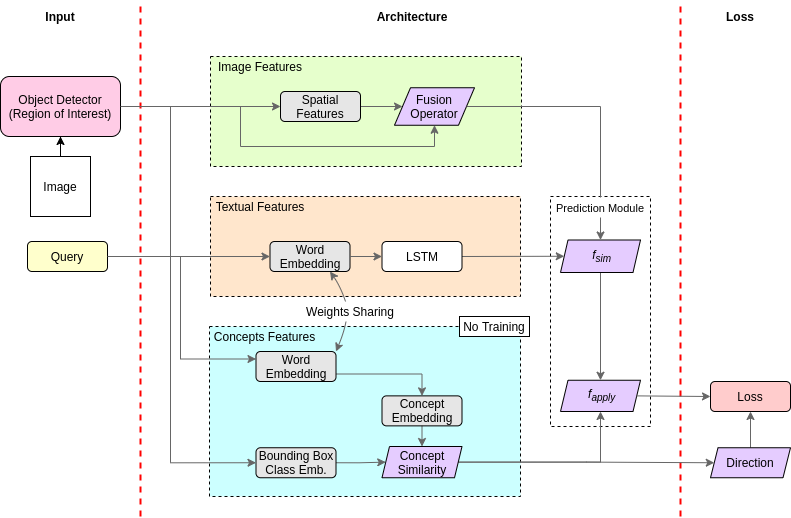
\includegraphics[width=1.0\textwidth]{figures/model-architecture.png}
    \caption[TODO]{Our model architecture overview. [WORK IN PROGRESS]}
    \label{fig:model-architecture}
  \end{figure}

\subsection{Visual Branch}

Given an image $\bm{I}$, we extract a set of $k$ bounding box
proposals $\calP_{\bm{I}} = \{ \bm{p}_i \}^k_{i=1}$ by means of a
pre-trained object detector, where $p_i \in \Rset^4$, jointly with
features $H^v = \{ \bm{h}^v_i \}^k_{i=1}$, where $\bm{h}^v_i \in
\Rset^v$. The features represent the internal object detector
activation values before the classification layers and regression
layer for bounding boxes. Moreover, our model extracts the spatial
features $H^s = \{ \bm{h}^s_i \}^k_{i=1}$, where $\bm{h}^s_i \in
\Rset^s$ from all the bounding boxes proposals, with the spatial
features for the proposal $\bm{p}_i$ defined as:
\begin{equation}
  \bm{h}^s_i = \left[ \frac{x1}{wt}, \frac{y1}{ht}, \frac{x2}{wt}, \frac{y2}{ht}, \frac{(x2 - x1) \times (y2 - y1)}{wt \times ht}  \right]
\end{equation}
where $(x1, y1)$ refers to the top-left bounding box corner, $(x2,
y2)$ refers to the bottom-right bounding box corner, $wt$ and $ht$ are
the width and height of the image, respectively. Both visual and
spatial features are then concatenated, thus leading to a set of new
vectorial representations $H^{||} = \{ \bm{h}^{||}_{jz} \}_{j \in [1,
\ldots, m], z \in [1, \ldots, k]}$, where vectors $\bm{h}^{||}_{jz}$
are defined as:
\begin{equation}
  \bm{h}^{||}_{jz} = \Big( \bm{W}^{||} \left( \bm{h}^s_z || L1(\bm{h}^v_z) \right) + \bm{b}^{||} \Big) 
\end{equation}
where $||$ indicates the concatenation operator, $\bm{h}^{||}_{jz} \in
\Rset^c$, $\bm{W}^{||} \in \Rset^{c \times (s + v)}$ is a matrix
of weights, and $\bm{b}^{||} \in \Rset^c$ is a bias vector.

% We also assume that the object detector returns, for each $\bm{p}_i$,
% a probability distribution $Pr_{Cls}(\bm{p}_i)$ over a set $Cls$ of
% predefined classes, i.e. the probability for each class $\zeta \in
% Cls$ that the content of the bounding box $\bm{p}_i$ belongs to
% $\zeta$. This information is typically returned by most of the object
% detectors, and it will be used to define our novel loss function.
% \todo{UPDATE: to define our...}

\subsection{Textual Branch}

Regarding the textual features extraction, given a noun phrase
$\bm{q}_j$, initially all its words $W^{\bm{q}_j} = \{ w^{\bm{q}_j}_i
\}^l_{i=1}$ are embedded in a set of vectors $E^{\bm{q}_j} =
\{e^{\bm{q}_j}_i \}^l_{i=1}$ where $e^{\bm{q}_j}_i \in \Rset^w$, where
$w$ is the size of the embedding. Then, our model applies a LSTM
neural network to generate from the sequence of word embeddings only
one new embedding $\bm{h}^*_j$ for each phrase $\bm{q}_j$. This
textual features extraction is defined as:
\begin{equation}
  \bm{h}^*_j = L1(LSTM(E^{\bm{q}_j}))
\end{equation}
where $\bm{h}^*_j \in \Rset^t$ is the LSTM output of the last word in
the noun phrase $\bm{q}_j$ , and $L1$ is the L$1$ normalization
function.

\subsection{Similarity Branch}

Along with visual and textual features we also compute a similarity
score between noun phrases and bounding box class labels. Such score
is crucial for learning to ground, and for consistency with (Wang et
al., 2019), we name it concept similarity. 

% The
% idea behind this is straightforward: the more the noun phrase and the
% councept expressed throught the bounding box label are semantically
% similar, the more they are related. In a weakly-supervised scenario
% where we are missing the grounding information, to known whether a
% phrase and the concept that it expresses (i.e, the bounding box) are
% related is very important for the learning process. 

% Here, an
% assumption is made: the bounding box class label semantically define
% the content of the bounding box. 

Formally, given set of proposal $\calP^{\bm{I}}$ and a noun phrase
$\bm{q}_j$, we compute the concept similarity score for each proposal
$i$ and phrase $j$ as:
\begin{equation}
  \bm{S}^c_{ji} = \fsim \left( \xi, \ePI_i \right),
\end{equation}
where $\fsim$ is a similarity measure such us the cosine similarity,
$\ePI_i$ is the embedding of the class for the $i$-th proposal, and
$\xi$ is the embedding representing the concept of the noun phrase
$\qj$:
\begin{equation}
  \xi = \fagg(\Eqj, \EPI).
\end{equation}
Please note that we use the same notation for both phrases word
embeddings and proposal class embeddings, indeed we define $\EPI =
\{\ePI_i \}^{k}_{i=1}$ the set of embeddings representing the bounding
box class labels, where $\ePI_i$ is the embedding of the class label
for proposal $i$ predicted with maximum confidence by the object
detector. 

The new embedding $\xi$ can be computed with different strategies: for
example, we can simply compute the mean of all word embeddings in the
noun phrase:
\begin{equation}
  \fagg^{\text{mean}}(\Eqj, \EPI) = \frac{\sum^l_{i=1} \eqj_i}{| \Eqj |},
\end{equation}
or use only the last word as done in (Wand et al, 2019):
\begin{equation}
  \fagg^{\text{last}}(\Eqj, \EPI) = \eqj_l.
\end{equation}
More complex strategies, instead, take into account external
information, such us the similarity wrt proposal class embeddings.
Here, we compute the similarity between word in noun phrase and
proposal class embeddings and then we select one word in the noun
phrase with maximum similarity wrt the detected concept in proposal:
\begin{equation}
  \fagg^{\text{max}}(\Eqj, \EPI) = \max_{\eqj \in \Eqj} \{ \max g(\eqj) \},
\end{equation}
where
\begin{equation}
  g(\eqj) = \{ \fsim(\ePI, \eqj) \mid \ePI \in \EPI \}.
\end{equation}

\subsection{Prediction Module}

Finally, the model predicts the probability $\bm{P}_{jz}$ that a given
noun phrase $\qj$ is referrred to a proposal bounding box $\bm{p}_z$
as:
\begin{equation}
  \bm{P}_{jz} = \fsim ( \bm{h}^{||}_{jz} , \bm{h}^*_j ).
\end{equation}
Here, $c$ should be equal to $t$, where $c$ and $t$ are the dimensions
of $\bm{h}^{||}_{jz} \in \Rset^c$ and $\bm{h}^*_j \in \Rset^t$,
respectively.

As noted in (Kan et al, 2018), concept similarit is a direct
consequence of the intrinsic knwoledge convoyed by the object
detector. Such score can be useful to down-weight unrelated proposals.
Its effectiveness is due to the fact that the word embedding usually
captures the semantic similarity between concept in phrase and the
content of the bounding box, and thus, let the model focuses on
relevant proposals.


Hence, we can apply the concept similarity on previously computed
$\bm{P}_{jz}$ as:
\begin{equation}
  \bm{P}^*_{jz} = \fapplysim \left( \bm{P}_{jz} , \bm{S}^c_{jz} \right).
\end{equation}
For consistency with other sections, we show that $\bm{P}_{jz}$ is
equal to $\bm{P}^*_{jz}$ by instancing $\fapplysim$ with
$\fapplysim^{\text{one}}$, a funcion that simply ignore $\bm{S}^c$
matrix:
\begin{equation}
  \fapplysim^{\text{one}} (\bm{S}^c_{jz}, \bm{P}_{jz}) = \bm{P}_{jz}.
\end{equation}
Outside of this section, we use the notation $\bm{P}^*$ for referring
to the prediction matrix, and whether the concept similarity is
applied or not is an implementation detail.

The simplest strategy for applying the concept similarity to
previously computed predictions is by multiplying the two, treating
$\bm{S}^c_{jz}$ as a weight matrix:
\begin{equation}
  \fapplysim^{\text{prod}} (\bm{S}^c_{jz}, \bm{P}_{jz}) = \bm{S}^c_{jz} * \bm{P}_{jz}.
\end{equation}

At first glance, this approach seems very promising because we force
the model to return predictions ``on steroid'' when there is a
semantic relation between phrase and proposal or downweighted when no
similarity is found. However, this relies on the assumption that the
embedding space and similarity measure we are using for words
perfectly captures the semantic similarity between them, and this is
not true. Also, we assume that proposals are classified with no error
by the object detector, neither this is true. Under those hypotesis,
such application of concept similarity cannot be fruitful. 

An example my clarify our statement. We are given $\bm{S}^c \in
\Rset^{1 \times 2}$, $\bm{S}^c = [0.1, 0.2]$ for an example composed by a
phrase and two proposal, and we know that the bounding box to ground
with our prhrase is the first. The only way the model has to output
the first proposal as the best bounding box, i.e., the bounding box to
ground, is to predict a score $p_{0}$ which is at least the double of
$p_{1}$, because
\begin{equation}
  \bm{P}^* = [0.1 * p_{0}, 0.2 * p_{1}]
\end{equation}
where $p_{j} = \bm{P}[0, j]$, and 
\begin{equation}
\begin{split}
0.1 * p_{0} > 0.2 * p_{1} & \iff p_{0} >  \frac{0.2}{0.1} * p_{1} \\
  & \iff p_{0} > 2 * p_{1}.
\end{split}
\end{equation}
Thus, with such scores $\bm{S}^c$, when the model predicts $0.1$ for
$p_1$, it must learn to predict $> 0.2$ for $p_0$, when it predicts
$0.5$ for $p_1$, it must learn to predict $1.0$ for $p_0$ and when it
predicts a value $> 0.5$ for $p_1$ there is no way to predict a
greater score for $p_0$. In conclusion, it's very difficult to learn
to ground in such settings and given problems highlighted above.

A more convenient way of applying concept similarity to prediction is
instead to compute the mean between two. Eventually, we can also put a
weight on two terms in order to balance contributions. Formally,
$\fapplysim$ becomes:
\begin{equation}
  \fapplysim^{\text{mean}} (\bm{S}^c_{jz}, \bm{P}_{jz}) = (1 - \lambda) * \bm{S}^c_{jz} + \lambda * \bm{P}_{jz}.
\end{equation}

\section{Training}

In this section, we present our loss. For the sake of presentation, we
define in the following the loss terms referred to a single example.
The total loss is then obtained by summing up the contributions of all
examples in the training set.

Please note that in weakly-supervised settings, for a training example
$\left( \bm{I}, S \right)$ we are not given the query-proposal pair
set $\{ ( q^{gt}_j, p^{gt}_j ) \}^m_{j=1}$, where $m$ is the number of
noun phrases.
% Thus, how can instruct our model to learn without the ground truth?
% This problem is well known in literature: in \todo{CITE: align2ground}
% they enforces the score between a noun phrase and a proposal to be
% higher than a non-paired proposal, and vice-versa. In ...
To tackle this problem, in our work we adopt a very simple strategy:
we exploit concept similarity. Basically, we consider ``positive'' an
example where the concept similarity is above a certain treshold, and
``negative'' an example whose concept similarity is below threshold:
\begin{equation}
  \bm{D}_{jz} =
  \begin{cases}
    0, & \bm{S}^c_{jz} > \sigma \\
    1, & \text{otherwise}
  \end{cases},
\end{equation}
 \todo{FIX: equation: out are in -1, 0, 1}
where $\bm{S}^c$ is the concept similarity. This policy relies on the
assumption that concept similarity correctly captures the semantic
relation between query and proposal. $\bm{D}$ is the concept direction
matrix.

Now, given a training example $\left( \bm{I}, S \right)$, where
$\cal{P}_{\bm{I}}$ the bounding box proposals set, we define the loss
function $\calL$ (for a single example) as:
\begin{equation}
  \calL = \frac{1}{m} \sum^m_{j=1} \Bigg( \frac{1}{z} \sum^k_{z=1} \floss ( \bm{P}^*_{jz}, \bm{D}_{jz} ) \Bigg)
\end{equation}
where $m$ in the number of noun phrases, $k$ is the number of proposal
bounding box, $\bm{P}^*_{jz}$ is the model predicted probability that
the noun phrase $\bm{q}_j \in \calQ$ refers to the image content
localized by $\bm{p}_z \in \calP_{\bm{I}}$. Our loss is scaled by $m$
and $k$ because number of noun phrase can change, but also number of
proposal: in our case, we ignore proposal with class label equal to
``background'' (see Sec.~\todo{REF: sec}). In the end, $\floss$ is the
function that optimize the learning process by combining predicted
scores with the concept direction. TODO: many strategie can apply, but
we chose...\todo{TODO: complete sentence}
\begin{equation}
  \floss ( \bm{P}^*_{jz}, \bm{D}_{jz} ) = -1 * ... % TODO \bm{D}_{jz} * x_pos + torch.square(y * x_neg)
\end{equation}
\todo{FIX: equation}

\end{document}
